\chapter{How I Turned \$1{,}000 Into \$1 Billion}

These companion notes follow a School of Hard Knocks interview with Glen Boyd, curated for this volume by LazyingArt LLC. We read the interview not as folklore about a lucky founder, but as a lecture on commercial transformation: an analytic engine is built for one domain, the market shifts, the same engine is redirected, proof arrives before theory, and then scale reveals a second layer of problems having to do with people, capital, and time.

\section{Outcome First, Then Origin}

We begin where the interview begins: not with biography, but with the compressed result. This is a deliberate choice. The lecture hands us the answer first, and only afterward asks us to reconstruct the mechanism.

\begin{align}
R_{1\,\mathrm{mo}} &= \$50{,}000,\\
R_{11\,\mathrm{mo}} &\approx R_{\mathrm{security}},\\
S_{4\,\mathrm{yr}} &= \$120\,\mathrm{M}.
\end{align}

These three lines are the solved puzzle. Within the first month, the new business is already nontrivial. Within eleven months, it is nearly matching the legacy security company. Within four years, it has become a very large enterprise. The rest of the lecture is an explanation of how that compression could possibly be true.

Only then do we rewind. Glen Boyd describes a very early start: self-taught programming, a company founded in his early twenties, a dot-com-era public offering in 1999, and a later merger exit. The point of this opening rewind is not simply credentialing. It establishes two things that matter for everything that follows: first, that the speaker is genuinely technical; second, that he is speaking from inside one of the first great network transitions.

\section{From Security Product to Internet Pivot}

The founding company does not begin as a web-marketing company at all. It begins as a security product for internal networks. The institutions are serious ones: the Federal Reserve, major banks, and other financial organizations under pressure to create audit control as more activity becomes computerized. The original business is small in headcount, large in concentration, and already commercially sound.

\subsection{Question \& Answer}

\paragraph{Question.} How did he know this was the company to go all in on?

\paragraph{Answer.} The lecture answers by first undoing the premise. He did not begin with the final product at all. The serious thing was not a fixed idea, but a technical capability plus a willingness to change domains when the external world changed. The company becomes worth going all in on not because the first product is sacred, but because the founders recognize that the market has moved and that their underlying machinery can move with it.

What changes the field is the internet. Yahoo and Netscape are not mentioned as trivia. They are signals that the relevant network is no longer the local network inside a bank, but the networked public world. Glen's train metaphor does important work here: a future is already moving, people are already aboard, and the real question is whether one can catch the last car before it disappears.

We can write the conceptual pivot in the simplest possible form. Let \(A\) denote the traffic-analysis engine they already possess. Let \(T_{\mathrm{LAN}}\) denote internal local-area-network traffic and \(T_{\mathrm{web}}\) anonymous inbound web traffic. Then the business changes by changing the domain and the output while preserving the analytic core:
\begin{align}
A(T_{\mathrm{LAN}}) &\mapsto \mathcal{R}_{\mathrm{sec}},\\
A(T_{\mathrm{web}}) &\mapsto \mathcal{R}_{\mathrm{mkt}}.
\end{align}

Here \(\mathcal{R}_{\mathrm{sec}}\) is a security or fraud report, and \(\mathcal{R}_{\mathrm{mkt}}\) is a marketing or audience-interest report. This is the lecture's central move. The founders do not throw away the engine; they change the question the engine is asked to answer.

\begin{figure}[h]
\centering
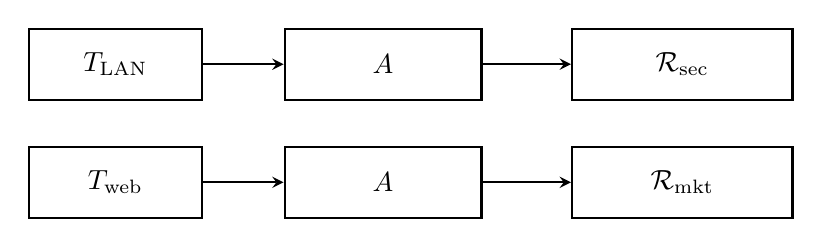
\begin{tikzpicture}[>=stealth,thick]
\node[draw,rectangle,minimum width=2.2cm,minimum height=0.9cm] (lan) at (0,1.5) {$T_{\mathrm{LAN}}$};
\node[draw,rectangle,minimum width=2.5cm,minimum height=0.9cm] (a1) at (3.4,1.5) {$A$};
\node[draw,rectangle,minimum width=2.8cm,minimum height=0.9cm] (sec) at (7.2,1.5) {$\mathcal{R}_{\mathrm{sec}}$};

\node[draw,rectangle,minimum width=2.2cm,minimum height=0.9cm] (web) at (0,0) {$T_{\mathrm{web}}$};
\node[draw,rectangle,minimum width=2.5cm,minimum height=0.9cm] (a2) at (3.4,0) {$A$};
\node[draw,rectangle,minimum width=2.8cm,minimum height=0.9cm] (mkt) at (7.2,0) {$\mathcal{R}_{\mathrm{mkt}}$};

\draw[->] (lan) -- (a1);
\draw[->] (a1) -- (sec);
\draw[->] (web) -- (a2);
\draw[->] (a2) -- (mkt);
\end{tikzpicture}
\caption{The lecture's pivot in compact form: the analytic core remains, while the traffic source and report type change.}
\end{figure}

The Sports Illustrated example tells us why this new output matters. A website can have a large number of visits for very different reasons, and raw volume alone is not enough to distinguish them. Let \(U\) denote the number of unique visitors, let \(f\) denote mean repeat-visit frequency, and let \(V\) denote total visits. Then
\begin{equation}
V = U\cdot f.
\end{equation}

\paragraph{Worked example.} Two traffic patterns can be equal in raw count and utterly different in market meaning:
\begin{align}
V_1 &= 100{,}000\times 1 = 100{,}000,\\
V_2 &= 10{,}000\times 10 = 100{,}000.
\end{align}

In the first case we have broad reach; in the second we have a smaller but highly repetitive audience. The web customer wants to know which world he is in. This is why the new output is not a security report but a marketing report. The same computational strength is now monetized by turning anonymous web traffic into interpretable demand.

\section{Proof Before Funding}

Once the pivot story has been told, the interview moves to funding. The host asks the standard startup question: how does one get money for an idea? Glen's answer is to reformulate the problem. Capital does matter, but it does not come first. Evidence comes first.

\subsection{Question \& Answer}

\paragraph{Question.} How do we get funding when all we have is an idea?

\paragraph{Answer.} We move as quickly as we can away from the mere idea and toward something demonstrable. In the lecture, the real variable is not rhetorical elegance but observable proof.

A compact way to write the lecture's logic is
\begin{equation}
\text{idea}\to \text{demo}\to \text{early adoption}\to \text{investable company}.
\end{equation}

This is not a theorem about all capital markets, but it is the lecture's governing update rule. The weaker the evidence, the harder the funding conversation. The stronger the evidence, the less the founder is asking the investor to believe on faith.

\begin{enumerate}
\item An idea alone is difficult to price.
\item A sample product is stronger because it can be demonstrated.
\item Early adoption is stronger still because the market has begun to speak.
\item Investor confidence rises when actual use can be shown rather than merely asserted.
\end{enumerate}

The lecture then sharpens the point with the old expression about whether the dogs eat the dog food. This is not a joke line. It is the interview's criterion for product reality.

\section{When the Dogs Eat the Dog Food}

Advertising cannot rescue a product that nobody wants. A concept is not validated by how impressive it sounds, nor by how much energy was spent presenting it, but by whether users actually take it up. In the lecture's commercial vocabulary, this is product pull.

We can summarize the principle in plain form:

\begin{remark}
A product becomes real to the market when people use it, not when the founder merely describes it well.
\end{remark}

The examples are chosen carefully. YouTube begins with something as humble as cat videos. Instagram begins with something equally narrow: people sharing personal photos. The lecture's point is not that these starting points were grand. It is that they were usable.

\begin{figure}[h]
\centering

\includegraphics[width=0.62\textwidth]{lecture_132_figure_03.png}
\caption{Instagram as an early example of a simple use-case---personal photo sharing---whose importance lies in real user pull rather than conceptual grandeur.}
\end{figure}

This is why the interview keeps returning to early adoption. A small but sticky use-case is better evidence than a large but purely verbal ambition. Once the founder can say not only ``this is a good idea'' but also ``people are already gravitating toward it,'' the discussion changes. The market has begun to provide its own testimony.

\section{Balance, Partnership, and Risk}

The lecture then widens from product logic to founder capacity. This is an important change of scale. We are no longer talking only about whether a business model works; we are talking about what it costs a human being to carry it.

Glen describes life-work imbalance, divorce, and later serious health consequences, including a heart attack and triple bypass surgery. In other words, scale is not only a property of the company. It is also a stress applied to the founder's body, relationships, and attention. The lecture's language becomes more personal here, but the conceptual point is still structural: growth consumes human slack.

Partnership appears as the first institutional answer to this problem. A strong co-founder or partner provides more than morale. The lecture treats partnership as operational load-sharing:
\begin{itemize}
\item emergencies can be absorbed,
\item work can be divided,
\item decisions can be argued out rather than carried alone,
\item non-identical skills can be combined into a larger effective capability.
\end{itemize}

The risk story sharpens this further. Glen describes quitting his job, getting down to roughly the last \(\$1{,}000\) in the bank, selling his motorcycle, and then being carried a little further by his partner's personal money. The important thing is not merely that this was risky. It is that the lecture gives a clear risk heuristic: failure still leaves the possibility of employment, while refusing to try leaves the possibility of permanent regret.

So the chapter's first view of entrepreneurial risk is neither romantic nor purely numerical. It is bounded downside paired with potentially irreversible missed opportunity. That asymmetry explains why he takes the gamble even with a newborn on the way.

\section{Judgment Under Scale}

Once the lecture has established product pull, human strain, and risk tolerance, it moves into operating judgment. Here the material comes in a chain rather than a single theory.

First come leadership traits. Glen names three that matter when assembling a team:
\begin{itemize}
\item honesty,
\item intelligence,
\item the ability to take constructive feedback.
\end{itemize}

The feedback point is especially important because it includes the founder himself. The lecture's picture of early partnership is argumentative rather than harmonious. Strong disagreement is acceptable, even useful, provided it is in service of a better path forward rather than ego.

The worst financial decision is then defined not by a bad spreadsheet, but by violation of gut alignment: getting involved in a business one never really wanted to be in. The cost in the lecture is concrete---close to \(\$3\,\mathrm{M}\)---but the deeper lesson is that operational attention can be consumed by a project that should have been refused at the door.

The best financial decision is subtler. The company is profitable and growing, so the founders seek venture capital in order to expand faster. The courtship is expensive in time and attention. Venture capital then passes. In the lecture, this feels like rejection in the moment, but it turns into strategic advantage.

\begin{figure}[h]
\centering

\includegraphics[width=0.78\textwidth]{lecture_132_figure_05.png}
\caption{Pitch-room imagery near the discussion of venture-capital courtship; the lecture emphasizes the time cost of the courtship and the strategic consequence of a pass.}
\end{figure}

The point is not simply that ``VC is bad.'' The point is that the absence of outside capital imposes a discipline the founders might not otherwise have had. We can write the two key consequences compactly as
\begin{align}
\frac{dE}{ds} &> 0,\\
O_{\mathrm{founders,IPO}} &\approx 95\%.
\end{align}

The first line is only schematic, but it captures the lecture's warning that expenses scale along with the business. The second is a hard outcome: when the company ultimately goes public, founder ownership remains extraordinarily high. Thus the failed VC courtship has a delayed financial payoff because it preserves ownership and enforces frugality.

\subsection{Question \& Answer}

\paragraph{Question.} Why do strong employees begin to fail when the company grows?

\paragraph{Answer.} Because the company is not standing still while the person is being evaluated. The job itself is climbing in altitude. A good employee at one scale may be above his or her oxygen line at the next.

This is where the interview becomes most model-driven. Glen says that ``Into Thin Air'' helped him see the problem: some people can go higher than others before performance collapses, and the remedy is sometimes not to demand more but to bring the person back down the mountain.

We can express the core managerial idea as a threshold statement:
\begin{equation}
n>n^\* \Rightarrow \text{manager overload and failure}.
\end{equation}
Here \(n\) is managerial load and \(n^\*\) the maximum load that the current person can carry successfully.

\begin{figure}[h]
\centering
\begin{tikzpicture}[x=1cm,y=1cm,>=stealth,thick]
\draw[->] (0,0) -- (6.4,0) node[right] {$n$};
\draw[->] (0,0) -- (0,3.6) node[above] {performance};
\draw (0.3,0.5) .. controls (1.5,1.9) and (2.4,2.7) .. (3.2,3.0);
\draw (3.2,3.0) .. controls (4.0,2.9) and (4.8,1.9) .. (5.8,0.5);
\draw[dashed] (3.6,0) -- (3.6,3.2);
\node[below] at (3.6,0) {$n^\*$};
\end{tikzpicture}
\caption{A schematic capacity threshold: as load $n$ rises past $n^\*$, performance may fall even for someone who was previously excellent.}
\end{figure}

The juggling analogy says the same thing in a different language. A person who can juggle three balls, then four, then five, eventually reaches a level at which the whole system collapses. The managerial conclusion is practical: stop handing out balls, redistribute responsibility, or hire someone who has already operated at the next scale.

Only two book titles are named clearly in the transcript, and the second gives the market analogue of the same threshold logic. ``Crossing the Chasm'' says that early adopters do not automatically carry us into the broader market. There is a gap in between:
\begin{equation}
\text{early adopters}\;\big|\;\text{chasm}\;\big|\;\text{early majority}.
\end{equation}

\begin{figure}[h]
\centering
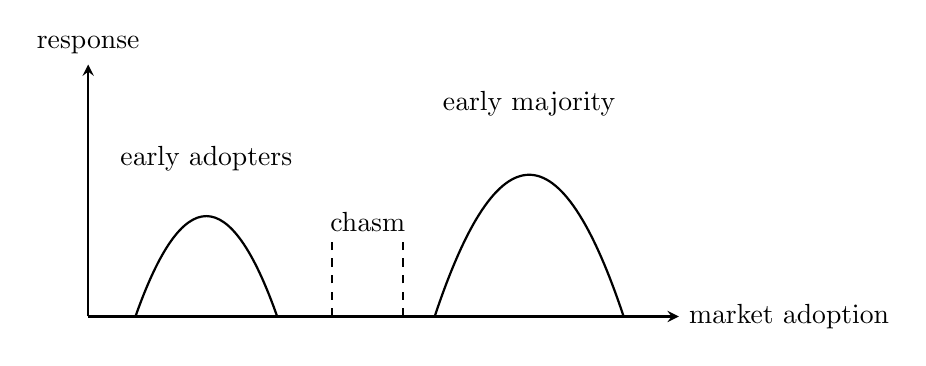
\begin{tikzpicture}[x=1cm,y=1cm,>=stealth,thick]
\draw[->] (0,0) -- (7.5,0) node[right] {market adoption};
\draw[->] (0,0) -- (0,3.2) node[above] {response};
\draw (0.6,0) .. controls (1.2,1.7) and (1.8,1.7) .. (2.4,0);
\draw (4.4,0) .. controls (5.2,2.4) and (6.0,2.4) .. (6.8,0);
\node at (1.5,2.0) {early adopters};
\node at (5.6,2.7) {early majority};
\node at (3.55,1.2) {chasm};
\draw[dashed] (3.1,0) -- (3.1,1.0);
\draw[dashed] (4.0,0) -- (4.0,1.0);
\end{tikzpicture}
\caption{A cautious schematic of the market gap described in the lecture's discussion of ``Crossing the Chasm''.}
\end{figure}

The first book models overload inside the company. The second models adoption outside the company. Together they explain why growth is hard even after product-market fit begins to appear.

\section{Reflection on Money, Happiness, and Time}

The lecture closes by narrowing from company mechanics to life valuation. Money, Glen says, does buy something real, but only up to a point. It buys relief from insecurity. It buys the ability to send children to college. It buys room to try things. Beyond that, the marginal increase in happiness tapers off. Better champagne is still champagne; better beaches are still beaches.

This section matters because it prevents the earlier numerical scale from becoming the whole measure of the chapter. The \(\$120\,\mathrm{M}\) in sales and the billion-dollar exit are real, but they are not the final theorem. The final theorem concerns what one should do with time.

The advice to the younger self is likewise not a single maxim. It is a cluster:
\begin{itemize}
\item enjoy life more,
\item take care of health earlier,
\item be less single-mindedly ambitious in ways that destroy relationships,
\item seek serious financial advice once success arrives.
\end{itemize}

The final exhortation against procrastination brings the lecture full circle. At the beginning we were given the result before the argument. At the end we are given the practical imperative before the reader can excuse delay. Time is the one nonrenewable resource. If we are going to fail, fail fast. If we are going to learn, learn early. If we wait for a perfect idea, we lengthen the path to any success that might have been reached by starting sooner.

\section{Summary}

The chapter's line of thought is now clear. A small security business becomes a large web-analytics business not by abandoning its technical core, but by redirecting it when the networked world changes. Funding follows proof rather than preceding it. User adoption is the decisive test. Scale then exposes a second layer of truths: expenses rise with size, managerial capacity has thresholds, adoption has thresholds, and the founder's own body and relationships are part of the system.

So the interview gives us more than a success story. It gives us a sequence of commercial models: preserve the core engine, change the question, look for proof, stay frugal, recognize human limits, and do not delay the attempt until time has already been spent.